\documentclass[10pt,aspectratio=169]{beamer}

% All the boilerplate is in deslides.sty
\usepackage{deslides}

\author{Ji\v{r}\'i Lebl}

\institute[OSU]{%
Oklahoma State University%
%Departemento pri Matematiko de Oklahoma {\^S}tata Universitato%
}

\title{2. Introduction to differential equations\\(Notes on Diffy Qs, 0.2)}

\date{}

\begin{document}

\begin{frame}
\titlepage

%\bigskip

\begin{center}
The textbook: \url{https://www.jirka.org/diffyqs/}
\end{center}
\end{frame}

\begin{frame}
Mathematics is the language of science, and differential equations
are the most basic and important part of it.

\medskip
\pause

You've already solved differential equations in calculus: You found
antiderivatives.

\medskip
\pause

Example you may not have seen:

{\small (Newton's law of cooling with variable ambient temperature)}
\[
\frac{dx}{dt} + x = 2 \cos t .
\]

\pause
$x$ is the \emph{dependent variable}

$t$ is the \emph{independent variable}

\medskip
\pause

It is a
\emph{first order differential equation}.

\end{frame}

\begin{frame}
What do we want do do with
\quad
$\displaystyle
\frac{dx}{dt} + x = 2 \cos t$ \quad ?

\medskip
\pause
We want to find a \emph{solution} $x$ in terms of $t$:
\quad
\pause
If we plug $x$ into the equation, it is satisfied.
\pause
\[
x = x(t) = \cos t + \sin t
\quad \text{is a solution.}
\]
\pause
Why?
\pause
\[
\frac{dx}{dt} + x
\pause
= 
\underbrace{(-\sin t + \cos t)}_{\frac{dx}{dt}}
+
\underbrace{(\cos t + \sin t)}_{x}
\pause
=
2\cos t .
\]
\pause
Yay!
\pause
\[
x = x(t) = \cos t + \sin t + e^{-t}
\quad \text{is also a solution.}
\]
\pause
\[
\frac{dx}{dt} + x
\pause
= 
\underbrace{(-\sin t + \cos t - e^{-t})}_{\frac{dx}{dt}} +
\underbrace{(\cos t + \sin t + e^{-t})}_{x}
\pause
= 2\cos t .
\]
\end{frame}

\begin{frame}
All solutions to 
\quad
$\displaystyle
\frac{dx}{dt} + x = 2 \cos t$ \quad are of the form
\[
x = \cos t + \sin t + C e^{-t}  \quad \text{($C$ is a constant)}
\]
\pause
\begin{center}
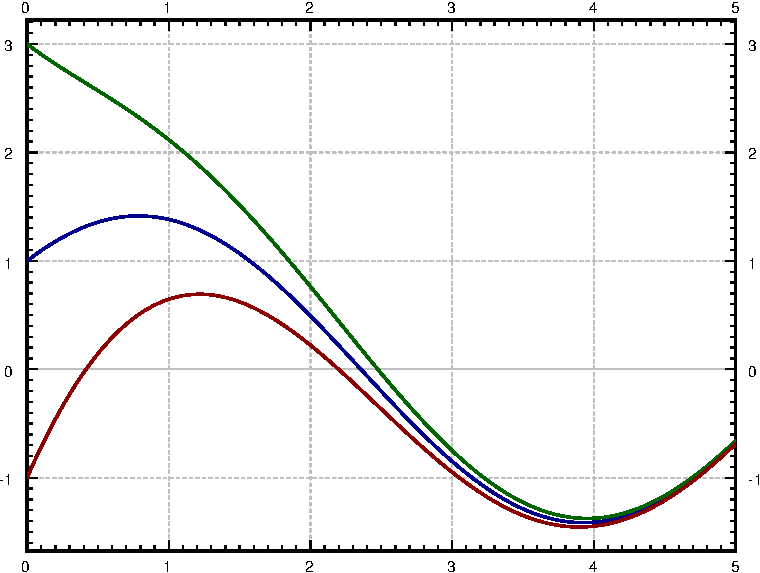
\includegraphics[width=2.9in]{../figures/intro-plots-alt}
\end{center}

\end{frame}

\begin{frame}
Finding solutions is hard: No completely general method.

\medskip
\pause

For simple cases we find exact analytic solutions.

\medskip
\pause

For complicated cases we may have to be satisfied with approximate, numerical
solutions.

\end{frame}

\begin{frame}

The entire process:

\pause
\medskip

\begin{center}
\scalebox{0.9}{
\subimport*{../figures/}{1-1-fig.pdf_t}
}
\end{center}
\end{frame}

\begin{frame}
\textbf{Example:} (Exponential growth model)

\medskip
\pause

$P$ population of bacteria in a Petri dish.

\medskip
\pause

At time 0, there is 100 bacteria, 10 seconds later there are 200.

\pause

Question: How many bacteria will there be at time 60 (1 minute)?

\medskip
\pause

Assume enough food and space.

\medskip
\pause

Rate of growth is proportional to the population, so our model is:
\pause
\[
\frac{dP}{dt} = kP \qquad \text{($k > 0$ constant)},
\]
\pause
Solution is \quad $P(t) = C e^{kt}$ \quad ($C$ a constant).

\medskip
\pause

Check: 
\quad
$\displaystyle
\frac{dP}{dt} \pause = C k e^{kt} \pause = k P$ \pause \quad {\Large\checkmark}

\end{frame}

\begin{frame}

Now what?  We have $P(t) = C e^{kt}$, but we don't know $C$ and we don't know $k$.

\medskip
\pause

We do know $P(0)=100$ and $P(10)=200$.

\medskip
\pause

$100 = P(0) \pause = C e^{k0} \pause = C$
\pause
\qquad
$200 = P(10) \pause = 100 \, e^{k10}$
\qquad
so
~
$2 = e^{10k}$ \pause ~or~ $k = \frac{\ln 2}{10} \approx 0.069$ 

\medskip
\pause

So
\quad
$P(t)=100e^{(\ln 2)t/10} \approx 100e^{0.069 t}$

\pause

\vspace*{-0.2in}

\hspace*{2.5in}
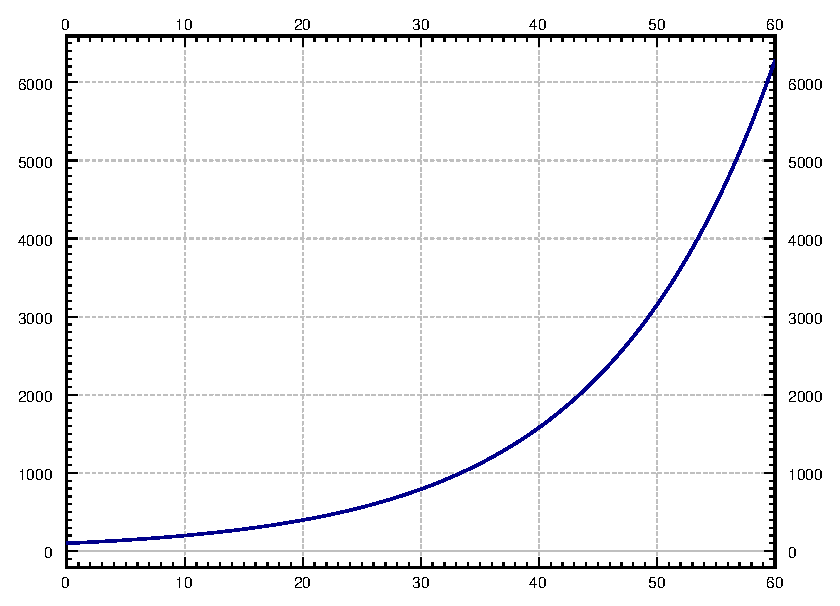
\includegraphics[height=2.05in]{../figures/intro-plotbact}

\vspace*{-1.8in}
\pause

$P(60) = 6400$

\pause

So at 1 minute there are 6400 bacteria.

\pause
\medskip

Exactly?

\pause
\medskip

At 61 seconds is there exactly

$P(61)\approx 6859.35$ bacteria?

\medskip
\pause

Obviously this is approximate.

\end{frame}

\begin{frame}

Typically $k$ is known and we solve one
\emph{initial condition} such as
$P(0)=100$ to get $C$.

\medskip
\pause

Example: Suppose $P' = P$ is the equation.

\medskip
\pause

$P(t) = C e^{t}$ \quad (giving \emph{all} solutions) is called the
\emph{general solution}.

\medskip
\pause

Given the initial condition $P(0) = 100$ the solution

\medskip

$P(t) = 100 \, e^{t}$ \quad is called the \emph{particular solution}.

\end{frame}

\begin{frame}
\textbf{Four fundamental equations:} ($y$ dependent variable, $x$ independent variable)

\medskip
\begin{enumerate}
\item\pause
$\displaystyle \frac{dy}{dx} = k y$, \quad $k > 0$

\medskip
\pause
General solution: \quad $y(x) = C e^{kx}$

\medskip
\item\pause
$\displaystyle \frac{dy}{dx} = -k y$, \quad $k > 0$

\medskip
\pause
General solution: \quad $y(x) = C e^{-kx}$

\medskip
\item\pause
$\displaystyle \frac{d^2y}{{dx}^2} = -k^2 y$, \quad $k > 0$

\medskip
\pause
General solution: \quad $y(x) = C_1 \cos(kx) + C_2 \sin(kx)$

\pause
\emph{second order differential equation} so two unknown constants $C_1$ and $C_2$.

\medskip
\item\pause
$\displaystyle \frac{d^2y}{{dx}^2} = k^2 y$, \quad $k > 0$

\medskip
\pause
General solution: \quad $y(x) = C_1 e^{kx}  + C_2 e^{-kx}$
\pause
\quad or \quad $y(x) = D_1 \cosh(kx) + D_2 \sinh(kx)$

\end{enumerate}

\end{frame}

\begin{frame}
For those that have not seen $\sinh$ and $\cosh$, the
\emph{hyperbolic sine} and \emph{hyperbolic cosine}:
\[
\cosh x = \frac{e^{x} + e^{-x}}{2} , \qquad
\sinh x = \frac{e^{x} - e^{-x}}{2} .
\]
\pause
Some properties:
\[
\cosh 0 = 1,
\pause
\quad
\sinh 0 = 0,
\pause
\quad
\frac{d}{dx} \cosh x = \sinh x,
\pause
\quad
\frac{d}{dx} \sinh x = \cosh x.
\]

\medskip
\pause
\textbf{Remark:} The shape of the graph of $\cosh$ is called a \emph{catenary}.
The arch in Saint Louis is an inverted $\cosh$:
\begin{equation*}
y = -127.7 \; \textrm{ft} \cdot \cosh({x / 127.7  \; \textrm{ft}}) + 757.7 \;
\textrm{ft} .
\end{equation*}


\end{frame}

\begin{frame}
Here are the graphs of $\sinh$ and $\cosh$:

\begin{center}
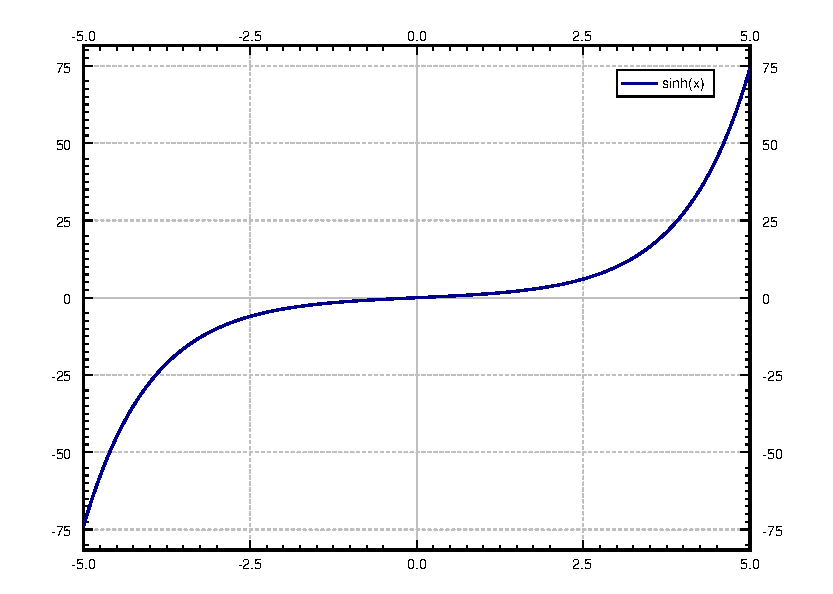
\includegraphics[width=2.65in]{figures/sinh.pdf}\quad%
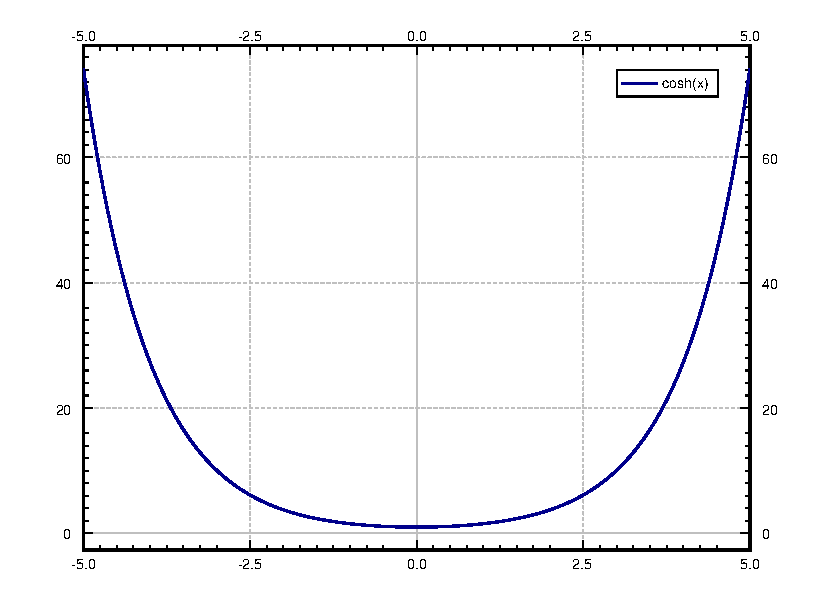
\includegraphics[width=2.65in]{figures/cosh.pdf}
\end{center}

\end{frame}

\begin{frame}
Compare with the graphs of exponential growth $e^x$ and exponential decay
$e^{-x}$

\begin{center}
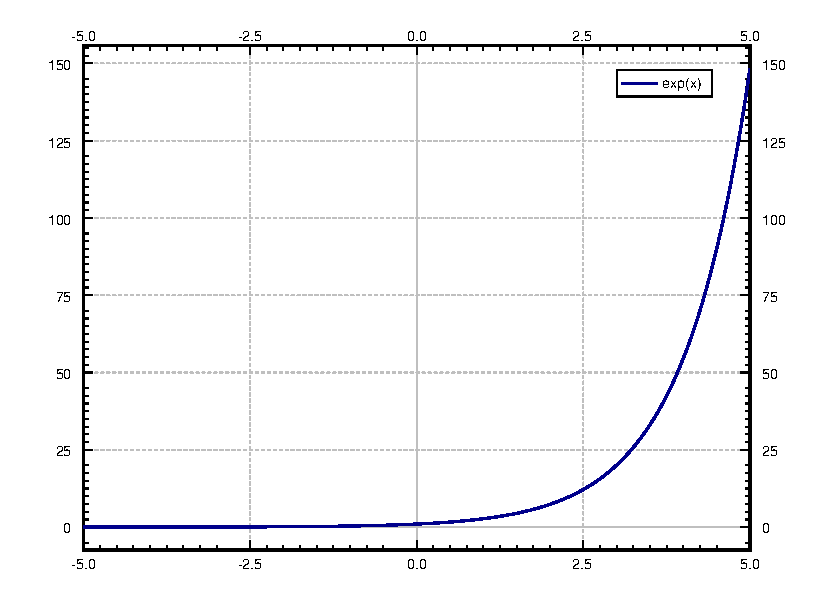
\includegraphics[width=2.65in]{figures/exp.pdf}\quad%
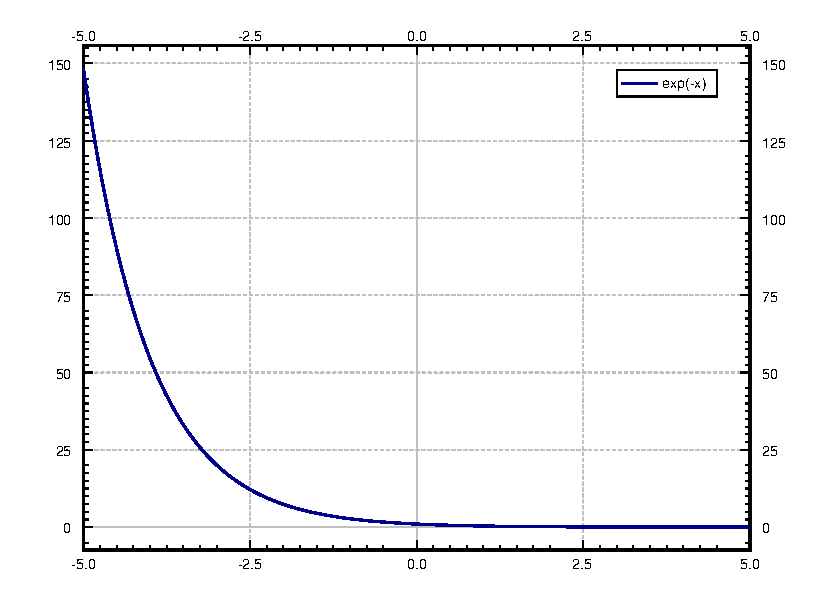
\includegraphics[width=2.65in]{figures/expdec.pdf}
\end{center}

\end{frame}

\begin{frame}
Just for completeness here are the graphs of $\sin$ and $\cos$:

\begin{center}
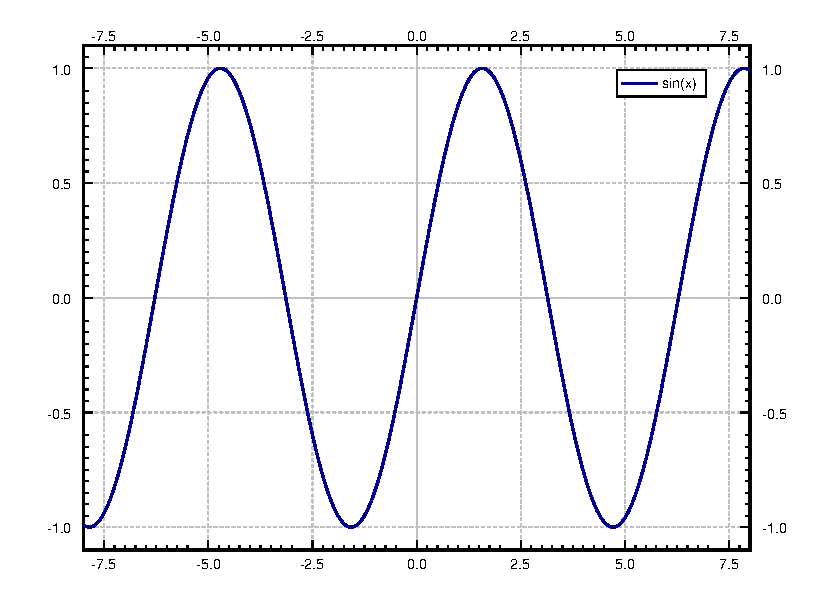
\includegraphics[width=2.65in]{figures/sin.pdf}\quad%
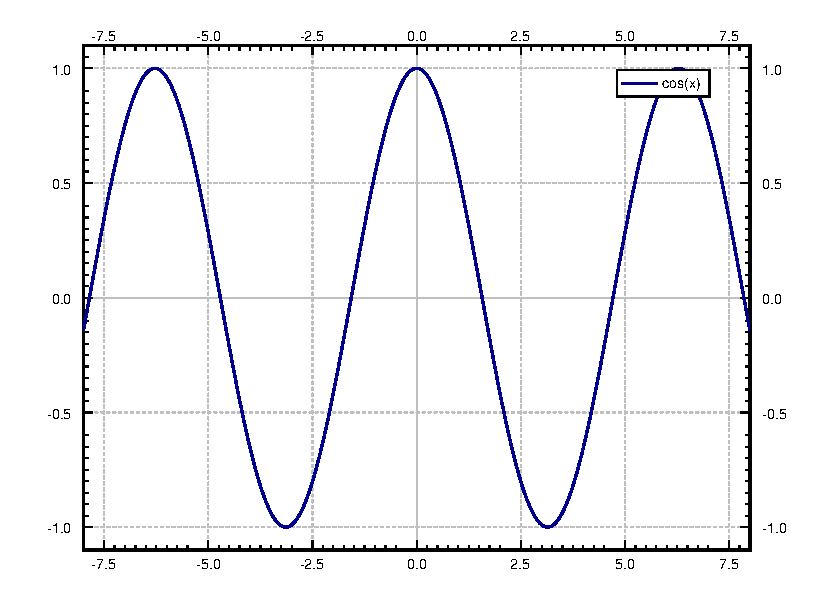
\includegraphics[width=2.65in]{figures/cos.pdf}
\end{center}

\end{frame}

\end{document}
